\documentclass[10pt]{article}
\usepackage[margin=0.75in]{geometry}
\usepackage{amsmath, amsthm, amssymb}
\usepackage{mathtools}
\usepackage{hyperref}
\usepackage{url}

\usepackage{enumitem}
\usepackage{setspace}
\usepackage{scalefnt}

\usepackage{titlesec}
\titlelabel{\thetitle.\quad}

\RequirePackage{fix-cm}

\usepackage{nicematrix}

\usepackage{mdframed}
\mdfdefinestyle{bframe}{%
    outerlinewidth=1pt,
    innertopmargin=0,
    innerbottommargin=5pt,
    innerrightmargin=8pt,
    innerleftmargin=8pt,
    backgroundcolor=white
   }
  
\usepackage{scalerel}
%\newcommand\plus{\scaleobj{0.5}{+}}


\newcommand{\+}{%
	\raisebox{0.18ex}{\scaleobj{0.55}{+}}
%  \raisebox{\dimexpr(\fontcharht\font`X-\height+\depth)/2\relax}{\scaleobj{0.5}{+}}%
}

\DeclareMathOperator*{\argmax}{arg\,max}
\DeclareMathOperator*{\argmin}{arg\,min}

\DeclareMathSymbol{\shortminus}{\mathbin}{AMSa}{"39}

\usepackage{dsfont}

\newtheorem{proposition}{Proposition}
\newtheorem{definition}{Definition}
\newtheorem{corollary}{Corollary}
\newtheorem{remark}{Remark}
\newtheorem{lemma}{Lemma}

\newcommand{\inv}{^{\raisebox{.2ex}{$\scriptscriptstyle-1$}}}
\newcommand\sbullet[1][.5]{\mathbin{\vcenter{\hbox{\scalebox{#1}{$\bullet$}}}}}
\newcommand\numberthis{\addtocounter{equation}{1}\tag{\theequation}}
\newcommand{\bigzero}{\mbox{\normalfont\Large\bfseries 0}}
\newcommand{\rvline}{\hspace*{-\arraycolsep}\vline\hspace*{-\arraycolsep}}

\title{\vspace{-2.0em} \vspace{-0.5em}}
\author{Matt Piekenbrock}
\date{}

\begin{document}
\noindent



\section{Introduction}
\subsection*{Motivation}
Persistent homology is, as of this time of writing, a well-studied mathematical structure. From its unassuming history starting with postniov towers, the body of research created over the past two decades have established perisstence as not only an intrinsic quantity, but a useful tool. 
From **, ** , to **, applications abound with persistence; see for an survey. PH is more than just a homology inference tool.  

Since its inception, a popular application of persistence in data analysis is its use as a featurization tool. 
In machine learning, featurization is a means of converting various data representations to a vector format amenable for learning and enhanced training. Classical examples include word2vec in natural language processing, Scale-Invariant Feature Transform (SIFT) in computer vision, extended-connectivity fingerprints (ECFs) in used in chemical informatics and molecular modeling, etc. 
More recent results include transformers... 
% Also mention size functions, matching distances..
Through no small feat of engineering, many of these techniques have been incrementally improved and adapted throughout the past decades, and tend to do quite well in terms of their efficiency. As such, they have seen widespread-adoption from more scientific fields trying to harness their power. 
While certainly useful, one of the pitfalls with such featurizations if the difficulty that comes with interpretation. 
% However, grasping the interplay between input features and their local contribution to NNP is growingly evasive due to heavy featurization
Difficulty in heavy featurization has lead to qualitative comparisons in scientific fields of the featurization outputs. Many are lead by the same equation: exactly what isa featurization tool capturing that is so useful for training?

Persistent homology is, in some sense, a natural tool for featurization. persistence is a stable invariant that comes equipped mathematical guarentees; thus featurization of diagrams can be interpreted as mapping persistence diagrams to Euclidean space in such a way that maximally preserves the topological information conveyed by the diagram. 
Moreover, we also know persistence diagrams retain some amount of geometry, such as those of curvature sets and the quasi-isometry theorems in distributed persistence. These results suggest an inverse theory related to persistence. 
Indeed, a recent injectivity result shows that collections of persistence diagrams are sufficient to uniquely characterize data sets in 2- and 3-dimensions\footnote{}, establishes persistence as truly an intrinsic description of shape. 

In what follows, we introduce a relaxation of the persistent Betti number (PBN) invariant that has certain advantages. Namely, we showing that a simple augmentation of traditional PBN computation leads to a continuous relaxation that $(1+\epsilon)$-approximates the PBN. Moreover, we show that this relaxation is permutation invariant, obeys and inclusion-exclusion principles, and admits a notion of stability in a certain sense---all properties useful in time-varying settings. 
Moreover, we show our relaxation is \emph{interpetretable} as it satisfies certain basic ``Betti-like'' properties and we illicit its connections back to spectral graph theory. 


%One of the 
%$<$ insert motivating examples, etc $>$

\subsection*{Related Work}





% Suppose one observes points in a geometric space whose position is driven by some unknown continuous-time system. 
% Towards understanding its dynamic, one may ask whether one can infer properties of the underlying evolving system
\section{Background \& Notation}\label{sec:background_notation}
% \textbf{Persistent Homology:}
A \emph{simplicial complex} $K \subseteq \mathcal{P}(V)$ over a vertex set $V = \{v_1, v_2, \dots, v_n \}$ is a collection of simplices $\{\sigma : \sigma \in \mathcal{P}(V) \}$ such that $\tau \subseteq \sigma \in K \implies \tau \in K$.
A \emph{filtration} $K_\bullet = \{K_i\}_{i\in I}$ of a simplicial complexes indexed by a totally ordered set $I$ is a family of complexes such that $i< j \in I \implies K_i \subseteq K_j$. $K_\bullet$ is called \emph{simplexwise} if $K_j \smallsetminus K_i = \{\sigma_j\}$ whenever $j$ is the immediate successor of $i$ in $I$ and $K_\bullet$ is called \emph{essential} if $i \neq j$ implies $K_i \neq K_j$:
%Connecting a sequence of simplices $[\sigma_i]_{i=1, \dots, m}$ ordered increasingly by $f$ by inclusion yields such a family of complexes:
\begin{equation}
	\emptyset = K_0 \subsetneq K_1 \subsetneq \dots \subsetneq K_m  = K_\bullet, \quad K_i  = K_{i-1} \cup \{\sigma_i\}
\end{equation} 
Filtrations may be equivalently defined as functions $f : K \to I$ satisfying $f(\tau) \leq f(\sigma)$ whenever $\tau \subseteq \sigma$. Here, we consider two index sets for $I$: $\mathbb{R}$ and $[n] = \{ 1, \dots, n\}$. 
Any finite filtration may be trivially converted into an essential, simplexwise filtration via a set of \emph{condensing}, \emph{refining}, and \emph{reindexing} maps~\cite{bauer2021ripser}. Thus, without loss of generality, we exclusively consider essential simplexwise filtrations and for brevity refer to them as filtrations.
%\\
%\\
%\noindent
%\textbf{Remark 1:}
%\normalfont In practice, filtrations often arise from triangulations parameterized by geometric scaling parameters. 
%%and references to the ``persistence'' of a given homology class are with respect to these parameterizations.
%For example, given a finite metric space $\mathcal{X} = (X, d_X)$, the \emph{Rips complex} at scale $\epsilon \in \mathbb{R}_{+}$ is defined as: 
%\begin{equation}
%	\mathrm{Rips_{\epsilon}}(\mathcal{X}) := \{ \sigma \subseteq X : d_X(x, x') \leq \epsilon \text{ for all } x, x' \in \sigma \} 
%\end{equation}
%\noindent Connecting successive complexes via inclusions $\mathrm{Rips_{\epsilon}}(\mathcal{X}) \hookrightarrow \mathrm{Rips_{\epsilon'}}(\mathcal{X})$ for $\epsilon < \epsilon'$ yields a family of complexes $\mathrm{Rips}_{\alpha} := \{ \, \mathrm{Rips}_\epsilon(\mathcal{X}) \, \}_{\epsilon \leq \alpha}$ called the \emph{Rips filtration}. 
%We keep the notation general by letting $K_\bullet$ denote any filtration. 
\\
\\
%As in equation~\eqref{eq:hom_map}, these inclusions induce linear maps at level of homology. Though we consider primarily Rips filtrations in this effort, we will at times keep the notation simple and general by letting $K_\bullet$ denote any simplicial filtration. 
For $K$ a simplicial complex and $\mathbb{F}$ a field, a $p$-chain is a formal $\mathbb{F}$-linear combination of $p$-simplices of $K$. The collection of $p$-chains under addition yields an $\mathbb{F}$-vector space denoted $C_p(K)$. 
The $p$-boundary $\partial_p(\sigma)$ of an oriented $p$-simplex $\sigma\in K$ is defined as the alternating sum of its oriented co-dimension 1 faces:
\begin{equation}\label{eq:alt_sum}
	\partial_p(\sigma) = \partial_p([v_0, v_1, \dots, v_p]) = \sum_{i=0}^p (-1)^i [v_0, \dots, \hat{v}_i, \dots v_p]
\end{equation}
where $\hat{v}_i$ indicates the removal of $v_i$ from the $i$th summand. Similarly, the $p$-boundary of a $p$-chain is defined linearly in terms of its constitutive simplices. 
A $p$-chain with zero boundary is called a $p$-cycle, and together they form $Z_p(K) = \mathrm{Ker}\,\partial_p$. Similarly, the collection of $p$-boundaries forms  $B_p(K) = \mathrm{Im}\,\partial_{p+1}$. Since $\partial_p \circ \partial_{p+1} = 0$ for all $p\geq 0$, the quotient space $H_p(K) = Z_p(K) / B_{p}(K)$ is well-defined, and $H_p(K)$ is called the $p$-th homology of $K$ with coefficients in $\mathbb{F}$. The dimension of the $p$-th homology group $\beta_p(K) = \mathrm{dim}(H_p(K))$ of $K$ is called the $p$-th \emph{Betti} number of $K$. 

Let $K_\bullet = \{K_i\}_{i\in [m]}$ denote a filtration of size $\lvert K_\bullet \rvert = m$. 
Let $\Delta_{+}^m = \{ (i,j) : 0 \leq i < j \leq m \}$ denote the set of valid pairs of filtration indices. 
For every such pair $(i,j) \in \Delta_{+}^m$, the inclusions $K_i \subsetneq K_{i+1} \subsetneq \dots \subsetneq K_j$ induce linear transformations $h_p^{i,j}$  at the level of homology:
\begin{equation}\label{eq:hom_map}
	0 = H_p(K_0) \to \dots \to H_p(K_i) \underbracket[0.5pt]{\to \dots \to}_{h_p^{i,j}} H_p(K_j) \to \dots \to H_p(K_m) = H_p(K_\bullet) 
\end{equation}
When $\mathbb{F}$ is a field, this sequence of homology groups admits a unique decomposition of $K_\bullet$ into a pairing of simplices $(\sigma_i, \sigma_j)$~\cite{} demarcating the evolution of homology classes: $\sigma_i$ marks the creation of a homology class, $\sigma_j$ marks its destruction, and the difference $\lvert i - j \rvert$ records the lifetime of the class, called its \emph{persistence}.
The $p$-th persistent homology groups are the images of these transformations and the $p$-th persistent Betti numbers are their dimensions:
\begin{equation}
	H_{p}^{i,j} = \begin{cases}
	H(K_i) & i = j \\ 
 	\mathrm{Im}\,h_p^{i,j} & i < j
 \end{cases}
, \quad \quad 
\beta_p^{i,j} = \begin{cases}
 	\beta_p(K_i) & i = j \\
 	\mathrm{dim}(H_{p}^{i,j}) & i < j
 \end{cases}
\end{equation}
For a fixed $p \geq 0$, the collection of persistent pairs $(i, j)$ together with unpaired simplices $(l, \infty)$ form a summary representation $\mathrm{dgm}_p(K_\bullet)$ called the \emph{$p$-th persistence diagram of $K_\bullet$}. Note that the persistent Betti numbers can be read off directly given $\mathrm{dgm}_p(K_\bullet)$; conceptually, $\beta_p^{i,j}$ simply counts the number of persistent pairs lying inside the box $[0, i] \times (j, \infty)$ (see Figure~\ref{})---the number of persistent homology groups born at or before $i$ that died sometime after $j$. 
\\
\\
% TODO: Define boundary matrix and matrix decompositions


%\begin{remark}
\textbf{Remark 2:} Persistence has been viewed from many different perspectives, and may be defined in a variety of ways. For example, Carlsson et al.~\cite{} observed persistence is simply a graded module under a particular polynomial ring. More recently, Baur studied persistence in a form a matching. Use follow the presentation from Cohen-Steiner et al~\cite{}: given a tame function $f: K \to \mathbb{R}$, its homological critical values $\{ a_i \}_{i=1}^n$, and an interleaved sequence $\{ b_i \}_{i=0}^n$ satisfying $b_{i-1} < a_i < b_i$ for all $i$, the $p$-th persistence diagram $\mathrm{dgm}_p(f) \subset \bar{\mathbb{R}}^2$ of a filtration induced by $f$ is defined as: 
\begin{equation}
\mathrm{dgm}_p(K_\bullet) = \{ \, (a_i, a_j) :  \mu_p^{i,j} \neq 0 \, \} \; \cup \; \mathcal{L}	
\end{equation}
%the set of points $(a_i,a_j)$ drawn on the plane with non-zero multiplicity $\mu_p^{i,j}$: 
where $\mathcal{L}$ denotes the points on the diagonal, counted with infinite multiplicity, and $\mu_p^{i,j}$ is defined as: 
\begin{equation}\label{eq:multiplicity}
	\mu_p^{i,j} = \left(\beta_p^{i,j\shortminus1} - \beta_p^{i,j} \right) - \left(\beta_p^{i\shortminus1,j\shortminus1} - \beta_p^{i\shortminus1,j} \right) \quad\quad \text{for } 0 < i < j \leq n+ 1
\end{equation}
where $\beta_p^{i,j}$ is the persistent Betti number defined at the values of the interleaved sequence, i.e. $\beta_p^{i,j} = \mathrm{dim}(\mathrm{Im}(h_p^{b_i, b_j}))$. More generally, by interpreting $\mu_p^\ast$ as function defined over $\bar{\mathbb{R}}$, Chazal~\cite{} view the multiplicity $\mu$ as a counting measure. This interpretation (as well as Cohen-Steiners) is perhaps the most relvent to the work we present here. 
%\end{remark}
%Although the persistence diagram $\mathrm{dgm}_p(K_\bullet)$ characterizes elements of $H_p^{i,j}$, one may define $\mathrm{dgm}_p(K_\bullet)$ through $\beta_p^{i,j}$ alone. To see this, let $f: K \to \mathbb{R}$ be a tame function and $(\tau_i)$
%\begin{definition}
%The $p$-th persistence diagram $dgm_p(f) \subset \bar{\mathbb{R}}^2$ of a filtration induced by $f$ is the set of points $(a_i,a_j)$ drawn on the plane with non-zero multiplicity $\mu_p^{i,j}$, where: 
%  $$\mu_p^{i,j} = \left(\beta_p^{i,j\shortminus1} - \beta_p^{i,j} \right) - \left(\beta_p^{i\shortminus1,j\shortminus1} - \beta_p^{i\shortminus1,j} \right) \quad\quad \text{for } 0 < i < j \leq n+ 1 $$
%\end{definition}



%\begin{definition}[Persistence diagram]
%	Given a finite filtration $K_\bullet$ of , the $p$-th persistence diagram for some $p \geq 0$ is the set of points $(i,j)$ counted with multiplicity $\mu_p^{i,j}$ for all $0 < i < j < m+1$, union all the points on the diagonal, counted with infinite .  
%\end{definition}


%Note that if $i = j$, then $H_{p}^{i,j} = H_{p}(K_i) = H_{p}(K_i)$ is   just the ``standard'' homology. 
% Simplices whose inclusion in the filtration creates a new homology class are called \emph{creators}, and simplices that destroy homology classes are   called \emph{destroyers}. 
% The filtration indices of these creators/destroyers are referred to as \emph{birth} and \emph{death} times, respectively. 
%The collection of birth/death pairs $(i,j)$ is denoted $\mathrm{dgm}_p(K)$, and referred to as the $p$-th \emph{persistence diagram} of $K$.
%If a homology class is born at time $i$ and dies entering time $j$, the difference $\lvert i - j \rvert$ is called the \emph{persistence} of that class.


\section{Methodology}
%We begin with a motivating application: suppose one has a dynamic point cloud that varies continuously with respect to some set of parameters and one expects this point cloud to have non-trivial topology as it changes. 
%Moreover, suppose one is interested in finding an a specific setting of parameter values wherein the $p$-th persistence diagram contains many highly persistent pairs; equivalently, one is interested in finding the parameter values where topological features are the most pronounced in the system's corresponding persistence diagram. in what follows, we make this problem statement and corresponding objective more precise towards developing an efficient tool for finding these parameter values. 
In what follows, we briefly outline the computation of the 

% For the moment, we omit the subscript $t \in \mathrm{T}$ and focus on a fixed instance of time. 
%\subsubsection*{Persistent Betti Numbers:} 
As in section~\ref{sec:background_notation}, let $B_p(K_\ast) \subseteq Z_p(K_\ast) \subseteq C_p(K_\ast)$ denote the $p$-th boundary, cycle, and chain groups of $K_\ast$, respectively. 
Given a simplicial filtration $K_{\bullet}$, let $\partial_p : C_p( K_{\bullet}) \to C_p(K_{\bullet})$ denote the boundary operator sending $p$-chains to their respective boundaries. 
With a slight abuse of notation, we also use $\partial_p$ to also denote the filtration boundary matrix with respect to an ordered basis $(\sigma_i)_{1 \leq i \leq m_p}$.  
The $p$-th persistent Betti number between scales $(i,j)$, $i < j$,  is defined as: 
\begin{align*} \label{eq:pbn}
	\beta_p^{i,j} &= \mathrm{dim}(H_p^{i,j}) \\
	&= \mathrm{dim} \left( Z_p(K_i) / (Z_p(K_i) \cap B_p(K_j) \right) \\
	& \numberthis = \mathrm{dim} \left( Z_p(K_i) \right) - \mathrm{dim}\left( Z_p(K_i) \cap B_p(K_j) \right ) 
\end{align*}
%Note that $\mathrm{dim}(C_p(K_\ast)) = \mathrm{dim}(B_{p-1}(K_\ast)) + \mathrm{dim}(Z_p(K_\ast))$ by the rank-nullity theorem, so we may rewrite~\eqref{eq:pb2} as:
%\begin{equation} \label{eq:pb3}
%\beta_p^{i,j} = \mathrm{dim} \left( C_p(K_i) \right) - \mathrm{dim} \left( B_{p-1}(K_i) \right) - \mathrm{dim}\left( Z_p(K_i) \cap B_p(K_j) \right )  
%\end{equation}
%The dimension of the boundary group $B_{p-1}(K_i)$ may be directly inferred from the rank of $\partial_p^{i}$, and the dimension of $C_p(K_i)$ is simply the number of $p$-simplices with filtration values $f(\sigma) \leq i$. 
While the dimension of $Z_p(K_i)$ is given by the dimension of the kernel of $\partial_p(K_i)$ and is thus easily computed, there are a variety of ways to address the computation of the intersection term (the persistence part). Zomorodian et al~\cite{} give a procedure to compute a basis for $Z_p(K_i) \cap B_p(K_j)$ via a sequence of Gaussian-elimination reductions. Conceptually intuitive alternatives for obtaining such basis is to use projectors, as studied by Ben Israel~\cite{}. 

We require more notation. If $A$ is a $m \times n$ matrix,
%then let $A^{i,j}$ denote the upper-left submatrix of $A$ given by the first $i$ rows ($j$ columns, resp.) and 
let $A^{i, j}$ denote the lower-left submatrix defined by last $m - i + 1$ rows (rows $i$ through $m$, inclusive) and the first $j$ columns, and let $A^{\ast, j}$ denote the submatrix given by including all $m$ rows and the first $j$ columns. 
%Given an $n \times m$ matrix $A$, let $A[I, J]$ refer to the submatrix formed by taking rows in the set $I$ and taking columns in the set $J \subseteq [m]$. Let $L_{, j}$
%\begin{equation}
%	\begin{bNiceMatrix}[first-row,first-col]
%       & i        & j \\
%i      & A & A_{ii}  \\
%m\text{ - }i & A_{\overline{i}i} & A_{jj}
%\end{bNiceMatrix}
%\end{equation}
\begin{figure}\label{fig:mult}
\centering
%	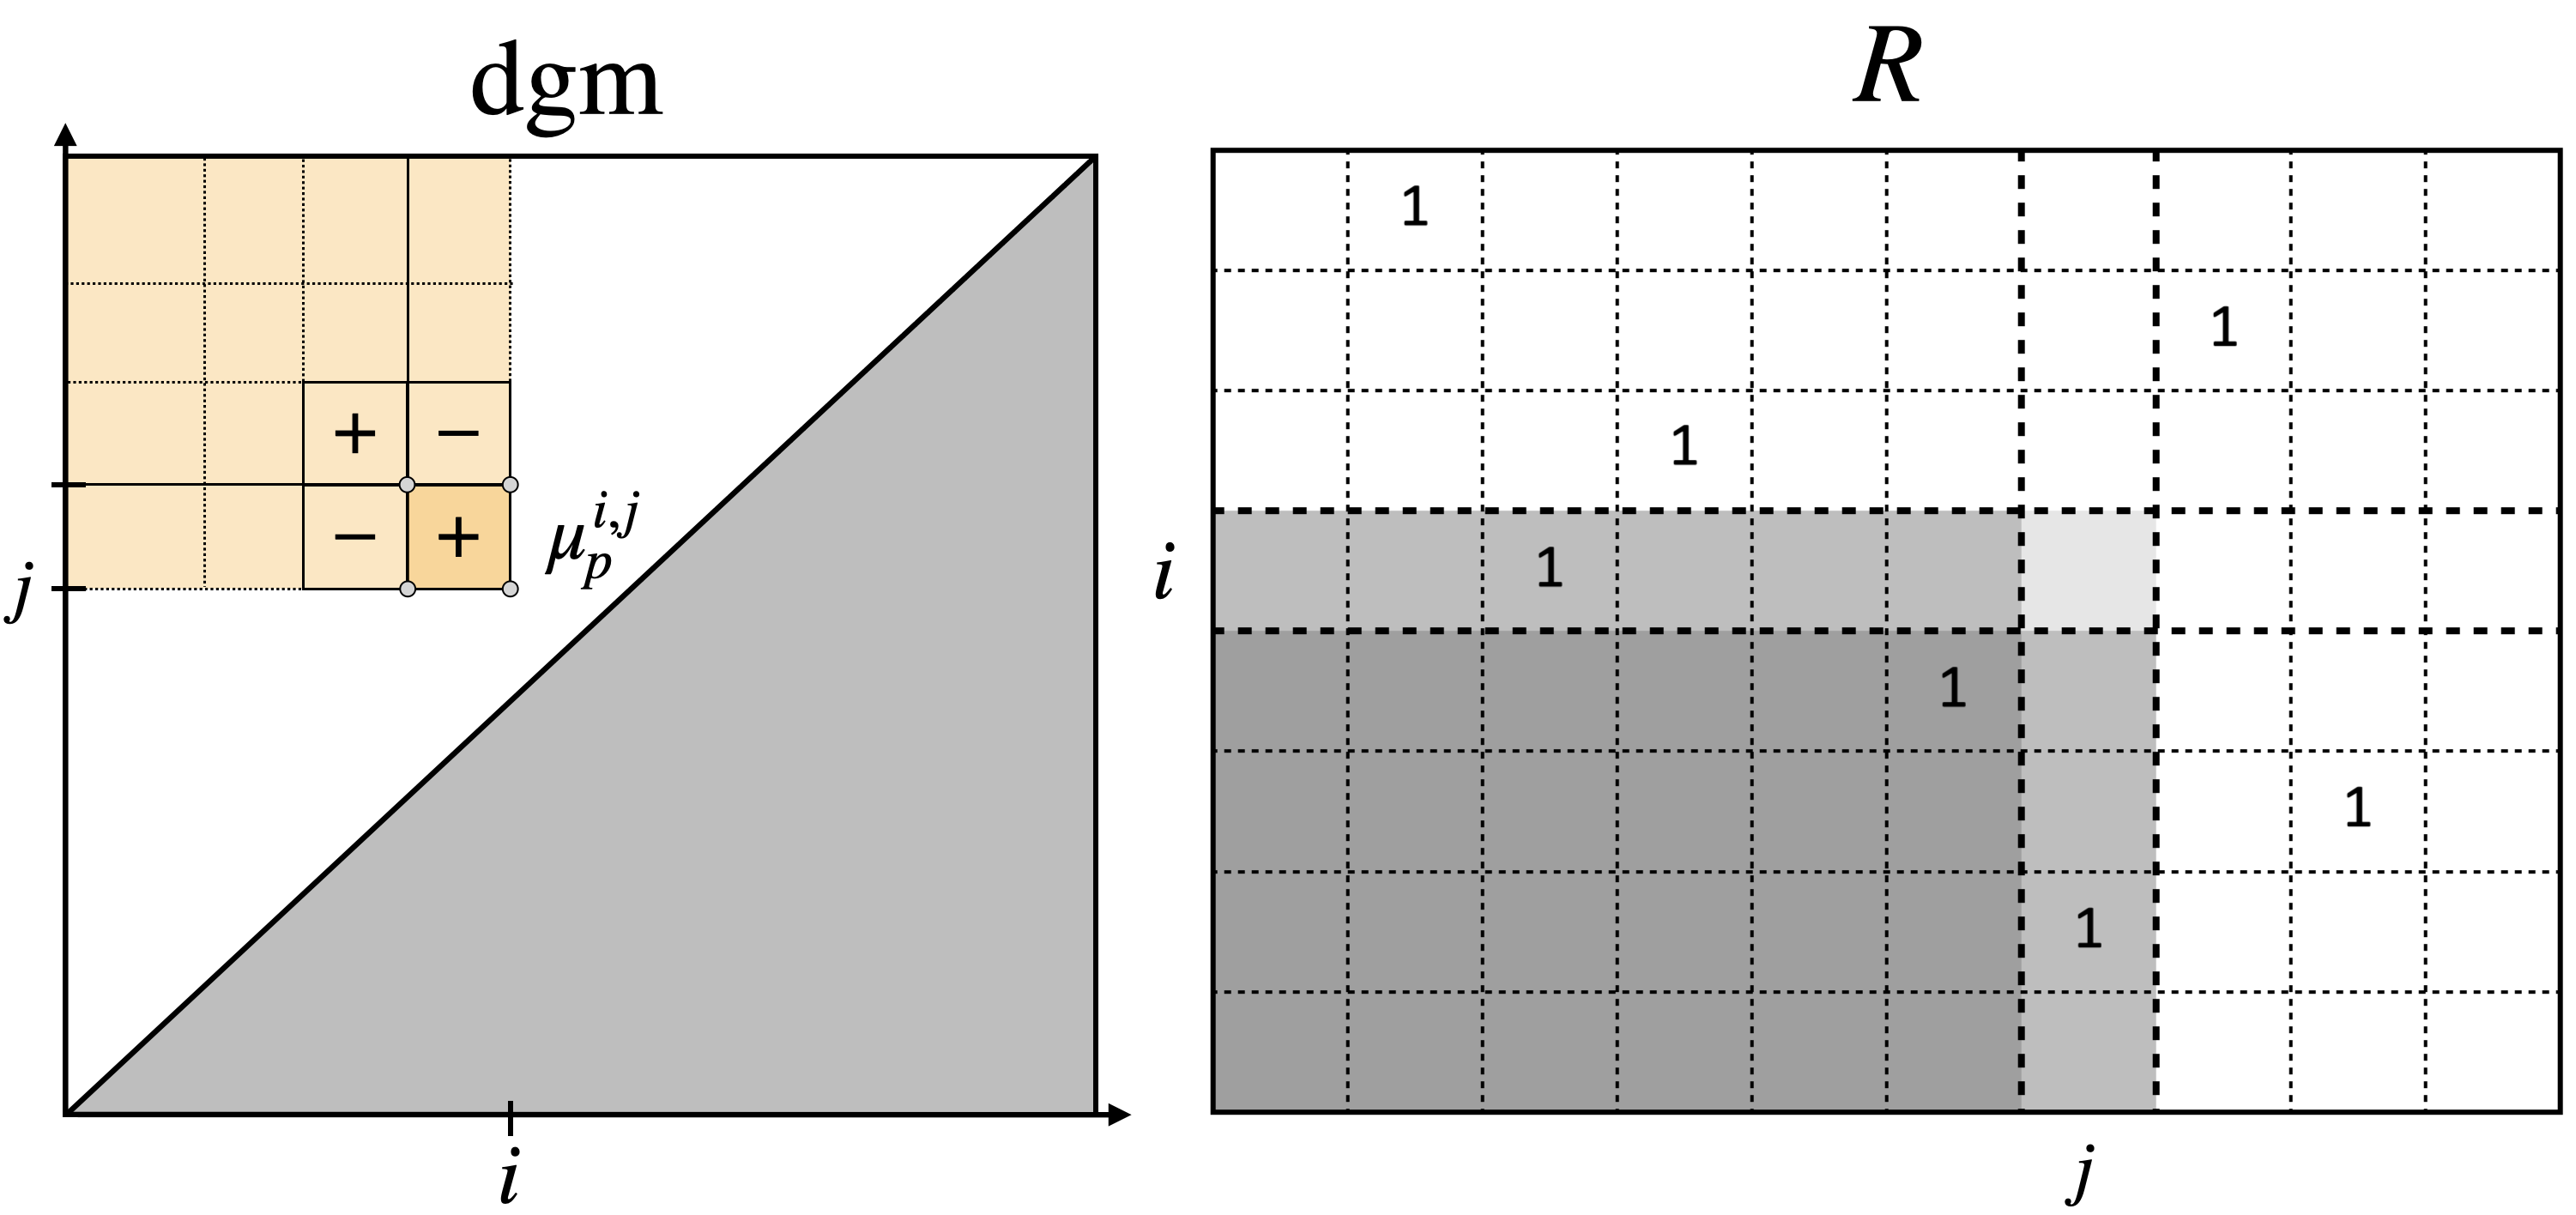
\includegraphics[width=0.45\textwidth]{mult_both}
	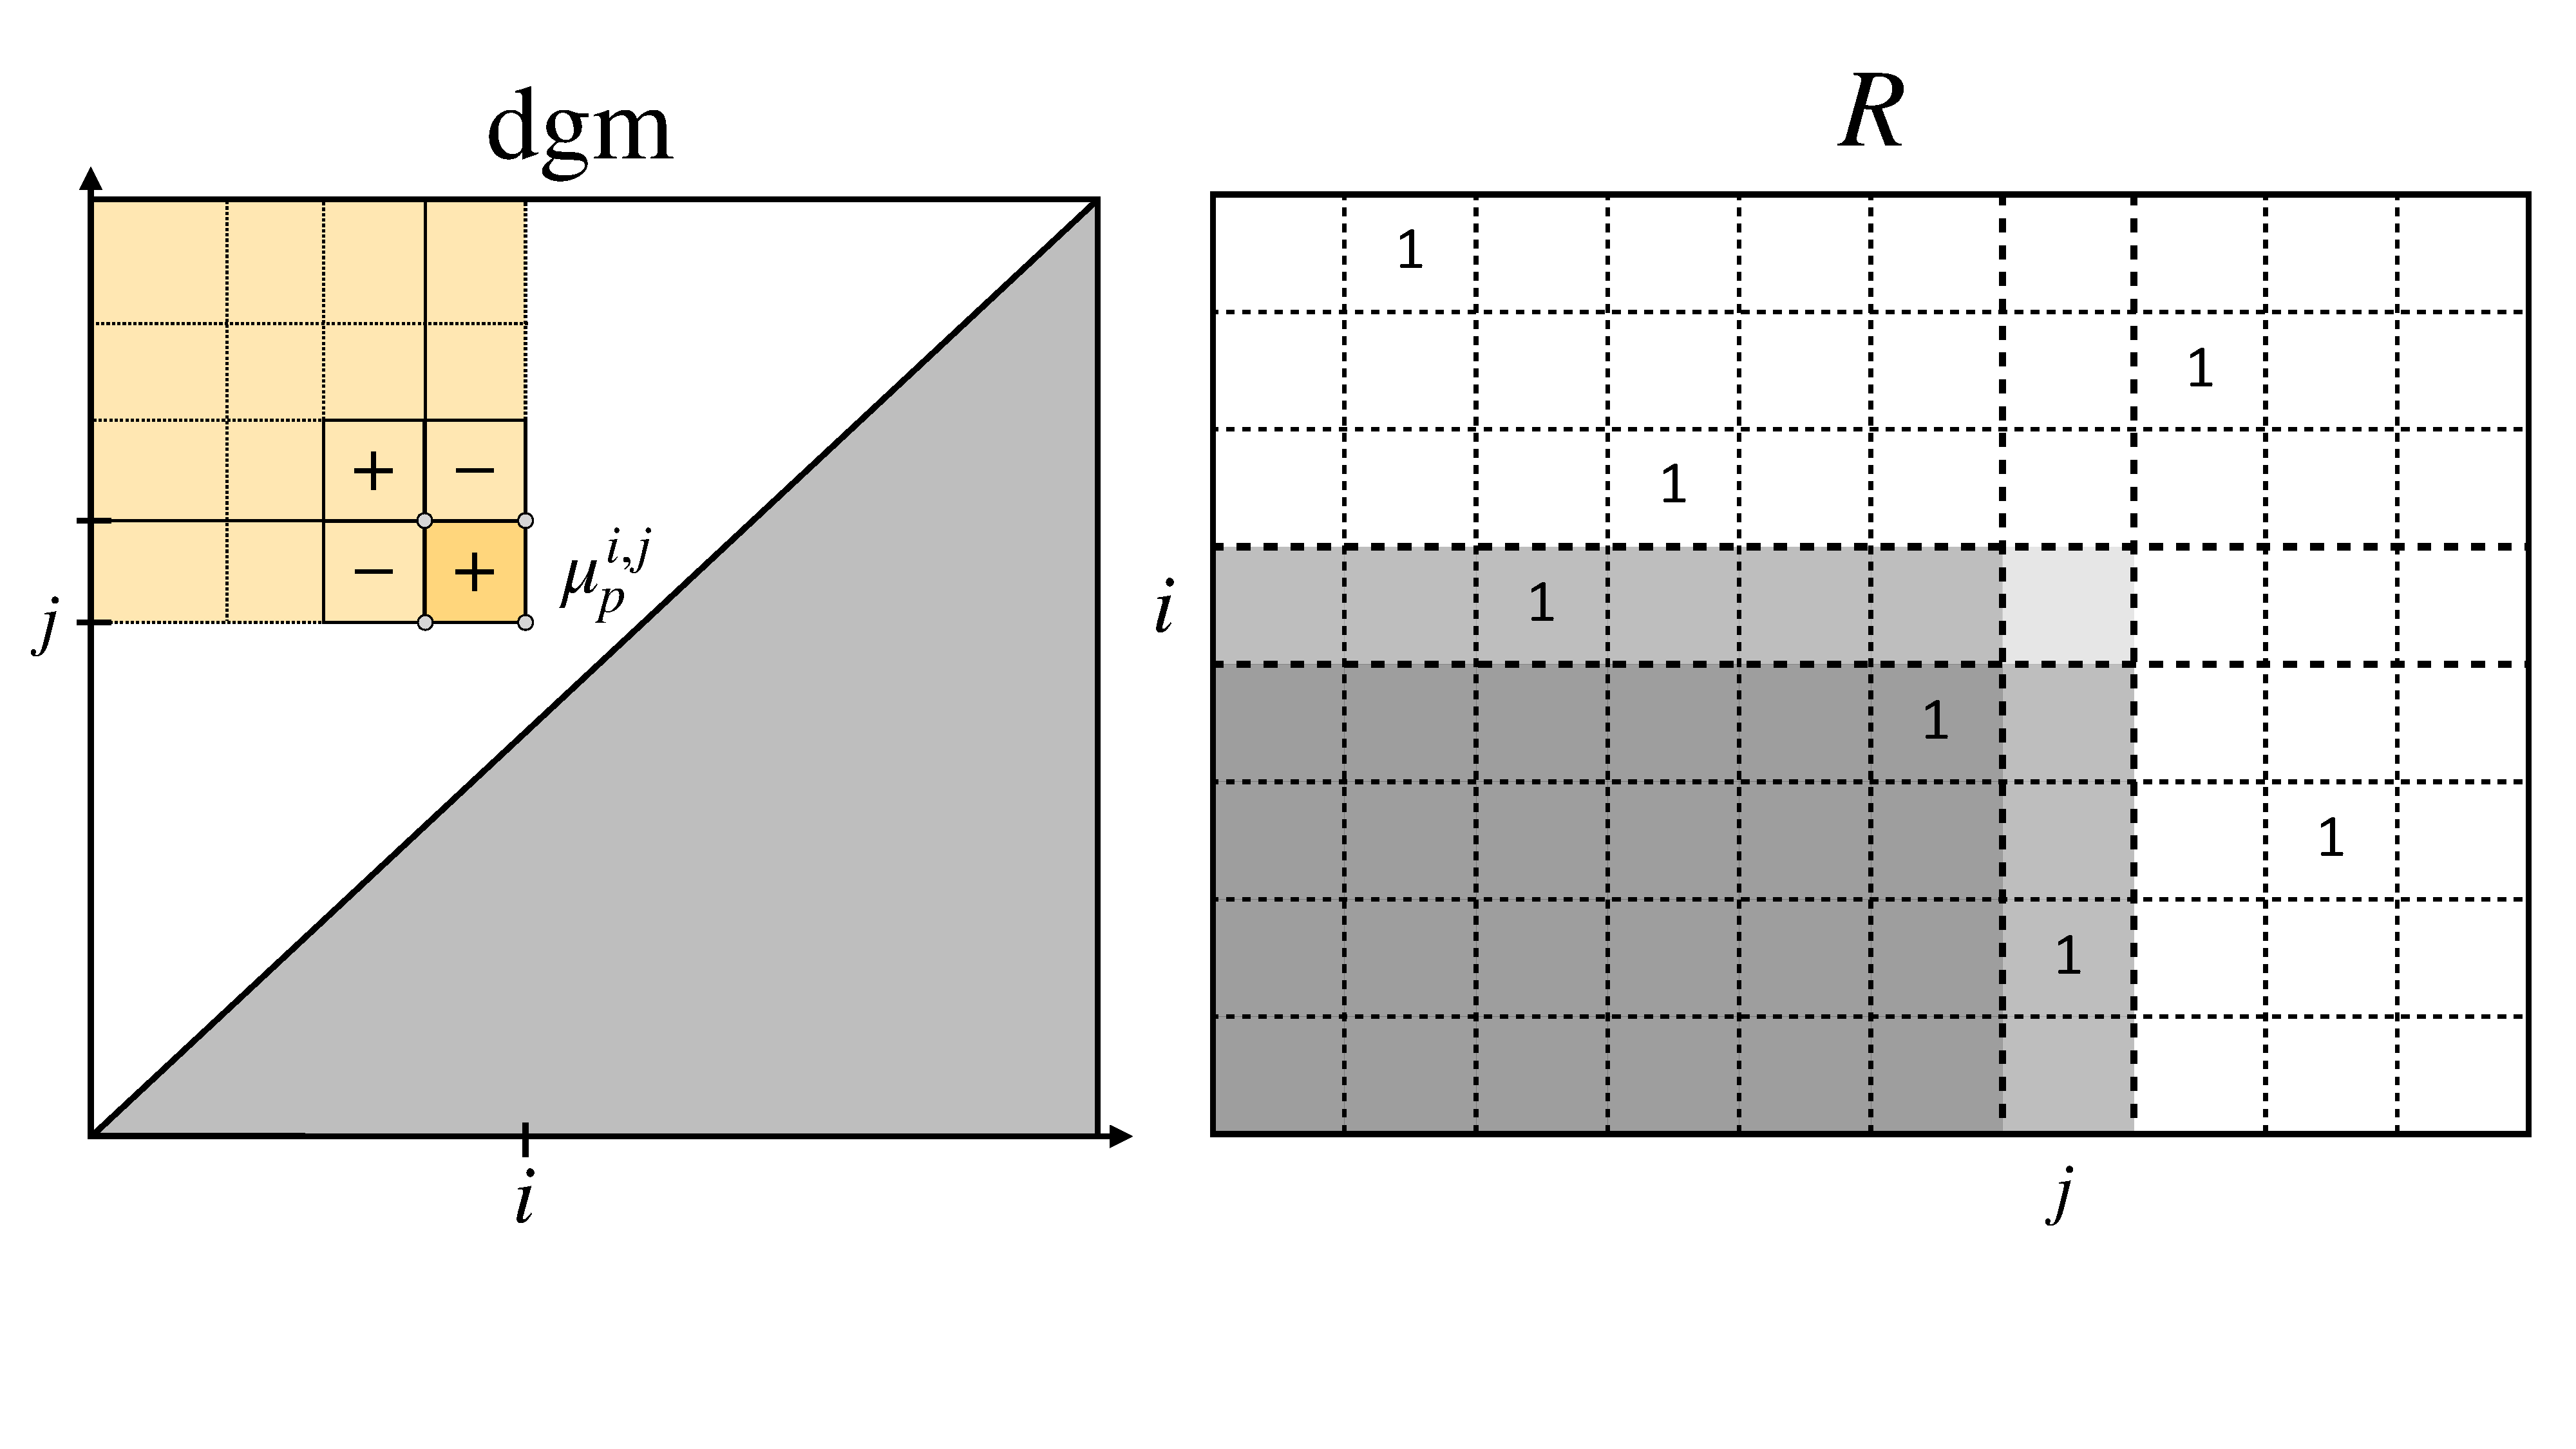
\includegraphics[width=0.45\textwidth]{pbsig_figs}
	\caption{Depicting the consequence of the inclusion-exclusion property of PBNs. Left: the multiplicity $\mu_p^{i,j}$ is given by cancellations of the PBNs, }
\end{figure}
For any $1 \leq i < j \leq m$, define $r_A(i,j)$ as follows:
\begin{equation}
	r_A(i,j) = \mathrm{rank}(A^{i,j}) - \mathrm{rank}(A^{i\texttt{+}1,j}) + \mathrm{rank}(A^{i\texttt{+}1,j\text{-}1}) - \mathrm{rank}(A^{i,j\text{-}1})
\end{equation}
%\begin{equation}
%	r_A(i,j) = \mathrm{rank}(A^{i, j}) - \mathrm{rank}(A^{i+1, j}) + \mathrm{rank}(A^{i+1, j-1}) - \mathrm{rank}(A^{i, j-1})
%\end{equation}
A consequence of the Pairing Uniqueness Lemma~\cite{} is that the quantity $r_R(i,j)$ has the effect of detecting whether $R[i,j] \neq 0$, see Figure~\ref{fig:mult}. In fact, the this lemma may be generalized to provide \emph{$\mu$-queries}, which count the number of . 
	Moreover, the structure theorem from~\cite{} shows that 1-parameter persistence modules can be decomposed in an \emph{essentially unique} way~\cite{}. 
As a result, we have our first lemma: 
\begin{lemma}\label{lemma:rank}
Let $R = \partial V$ denote the matrix decomposition of a given filtered boundary matrix $\partial$ derived from the associated filtration $K_\bullet$. For any pair $(i,j)$ satisfying $1 \leq i < j \leq m$, we have:
	\begin{equation}\label{eq:lower_left_rank}
		\mathrm{rank}(R^{i,j}) = \mathrm{rank}(\partial^{i, j})
	\end{equation}
Equivalently, all lower-left submatrices of $\partial$ have the same rank as their corresponding submatrices in $R$. 
\end{lemma}
Lemma~\ref{lemma:rank} was the essential motivating step used by Chen et al~\cite{} in their rank-based persistence algorithm, which was the first output-sensitive algorithm given for computing persistent homology of a filtered complex. We show this result allows us to write the persistent Betti number as a sum of rank functions defined over \emph{unfactored} matrices. 
\begin{proposition}
For some fixed $p \geq 0$, let $R_p = \partial_p V_p$ denote the reduced decomposition of the $p$-dimension boundary matrix $\partial_p$ of some filtration $K_\bullet$.  
%	\begin{equation}\label{eq:betti_four}
%	\beta_p^{i,j} = \mathrm{rank}(I_p^i) - \mathrm{rank}(\partial_p^{\ast,i}) - \mathrm{rank}(\partial_p^{i,j}) + \mathrm{rank}(\partial_p^{i+1,j})
%	\end{equation}
	\begin{equation}\label{eq:betti_four}
	\beta_p^{i,j} = \mathrm{rank}(I_p^{\ast,i}) - \mathrm{rank}(\partial_p^{\ast,i}) - \mathrm{rank}(\partial_{p\+1 }^{\ast,j}) + \mathrm{rank}(\partial_{p\+1}^{i \+ 1, j} )
	%\mathrm{rank}(\partial_{p+1}^{i+1,\ast} \otimes\partial_{p+1}^{\ast,j} )
	\end{equation}
where $I_p^{\ast,i}$ denotes the identity matrix with $i$ columns.
\end{proposition}
\noindent In conclusion, we may write the persistent Betti number as a combination of rank computations performed directly on the (ordered) dimension $p$ and $(p+1)$ boundary matrices. As we will show in the next section, this formulation has a few advantages over the approaches given by Zomorodian Carlsson, or the projector approaches~\cite{}. 
% DONT ERASE
%Let $\partial_p^{b}$ and $\partial_p^{b, d}$ denote matrices whose columns span the subspaces $B_{p-1}(K_b)$ and $Z_p(K_b) \cap B_p(K_d)$, respectively. We address their computation in section~\ref{sec:computation}. Substituting these matrices appropriately, equation~\eqref{eq:pb3} can be written as: 
%\begin{equation}\label{eq:pb_rank}
%	\beta_p^{b,d} = \lvert \, \partial_p^b \, \rvert - \mathrm{rank}(\partial_p^b) - \mathrm{rank}(\partial_{p+1}^{b,d}) 
%\end{equation}
%where $\lvert \, M \, \rvert = \mathrm{dim}(\mathrm{dom}(M))$. Thus, $\beta_p^{b,d}$ is expressible as a difference between a simple-to-compute quantity ($\lvert \, \partial_p^b \, \rvert$ simply counts the number of $p$-simplices with filtration value $f(\sigma) \leq b$ for some fixed $b \in \mathbb{R}_+$) and the rank of two particular matrices. We make use of this fact in later sections of the paper. 
% NOTE: Keep i,j as the indices in the notation for the above section; the next section makes clear the transition to \epsilon_i, \epsilon_j


\subsubsection*{A Time-varying Boundary Matrix Relaxation}
% Jordan canonical form 
Thus, we require alternative expressions for each of the terms in equation~\eqref{eq:betti_four} to extend its applicability to the time-varying setting. Towards deriving these expression, we first require a replacement of the standard boundary matrix formulation. 
% Give example of optimal homologus cycle 



Recall that the boundary operator $\partial_p$ for a finite simplicial filtration $K_{\bullet}$ with $m = \lvert C_p(K_{\bullet}) \rvert$ and $n = \lvert C_{p-1}(K_{\bullet}) \rvert$ can be represented by an $(n \times m)$ boundary matrix $\partial_p$ whose columns and rows correspond to $p$-simplices and $(p-1)$-simplices, respectively. The entries of $\partial_p$ depend on the choice of $\mathbb{F}$; in general, after orientating the simplices of $K$ arbitrarily, they have the form: 
%Given an oriented $p$-simplex $\sigma = [v_0, v_1, \dots, v_p]$, its corresponding image under the  boundary operator $\partial_p$ is given as: 
%\begin{equation}\label{eq:alt_sum}
%	\partial_p(\sigma) = \partial_p([v_0, v_1, \dots, v_p]) = \sum\limits_{i=0}^p (-1)^i [v_0, \dots, \hat{v}_i, \dots v_p]
%\end{equation}
%where $\hat{v}_i$ indicates the removal of $v_i$ from the $i$th summand.  
\begin{equation}\label{eq:matrix_pchain}
	\partial_p[i, j] = \begin{cases} 
	c(\sigma_j)  & \text{if } \sigma_i \in \partial_p(\sigma_j) \\
	0 & \text{otherwise}
   \end{cases}
\end{equation}
where $c(\sigma_\ast) \in \mathbb{F}$ is an arbitrary constant satisfying $c(\sigma) = -c(\sigma')$ if $\sigma$ and $\sigma'$ are opposite orientations of the same simplex, typically set to $\pm 1$.  Towards relaxing the persistent Betti computation in dynamic setting, we seek an alternative choice for $c(\sigma)$ which endows continuity in the entries of $\partial_p$ in $T$.

Observe that one of the consequence of the formulation~\ref{} with is that we may take advantage of the the various properties of the rank function. One such property is permutation invariance, i.e. $\mathrm{rank}(A) = \mathrm{rank}(P^T A P)$. Thus, we need not represent the boundary matrices $\partial_p$ in the filtration order. 
Moreover, unlike the vineyards algorithm~\cite{}, this also implies we do not need to \emph{maintain} the filtration order in the time-varying setting---as long as the matrices have the correct non-zero pattern as their filtered equivalents, the PBNs may be deduced via rank functions. 

% Change index sets 
We revisit the choice of index sets. 
We formalize this with the following definition.  

% $\delta_{\mathcal{X}}(\cdot) = (X, d_X(\cdot))$ a DMS over a finite set $X$ of fixed size $\lvert X \rvert = n$
\begin{definition}[Time-varying boundary matrix]\label{def:time_boundary_matrix}
Let $\mathbb{F} = \mathbb{R}$ denote the field, and let $(\mathcal{P}(X), \preceq^\ast)$ be a linear extension of the face poset of $K_\bullet$. For some constant $\omega > 0$, a time-varying $p$-th boundary matrix $\partial_p^t$ is an $\binom{n}{p} \times \binom{n}{p\+1}$ matrix whose entries $c(\sigma)$ satisfy:
$$
\partial_p^t[i,j] = \begin{cases}
	\pm \, S_{\omega}(\epsilon) & \text{if } \sigma_i \in \partial_p(\sigma_j), \text{ where } \epsilon = f(\sigma_j) \\
	0 & \text{otherwise}
\end{cases} 
% c(\sigma) = \lvert \epsilon - \mathrm{diam}_t(\sigma) \rvert_{+}
$$
where $S_{\omega, \epsilon}(\sigma_j)$ is a \emph{smooth-step} function whose range decreases smoothly from $1 \to 0$ in the interval $f(\sigma_j) \pm \frac{\omega}{2}$, and where rows and columns of $\partial_p^t$ follow fixed order given by $\preceq^\ast$ for all $t \in T$.% the image of a function $\partial_p^\ast: T \to \mathbb{R}^{k \times l}$ 
%and the total order on $K(\cdot)$ is fixed.  
\end{definition}
\noindent
We now show a few properties that $\partial_p^t$ exhibits which is advantageous for time-varying systems. Clearly the entries of $\partial_p^t$ must vary continuously in $t \in T$. Moreover, for fixed $p \geq 0$, we have:
% 
% Lipshitz statement about boundary matrix
% At the algebraic level, persistent homology admits a canonical decomposition for coefficients in any choice of field~\cite{}, though at the expense of torsion information.\footnote{}
% Given a strict total order $(V, <)$ on the vertices of $K$, define the ranking function $\varsigma_p(\tau) : K_p \to [m_p]$ which ranks the $p$-simplices of $K$ in a fixed way according to the order given by $<$. 
% If $\sigma$
%We begin by extending the standard definition of an elementary $p$-chain to the dynamic setting. Recall a $p$-chain of a simplicial filtration $K_\bullet$ with coefficients in $\mathbb{F}$ is a function $c_p$ on the oriented $p$-simplices of $K$ satisfying $c_p(\sigma) = -c_p(\sigma')$ if $\sigma$ and $\sigma'$ are opposite orientations of the same simplex, and $c_p(\sigma) = 0$ otherwise. 
%A $p$-chain is called \emph{elementary with respect to $q \in \mathbb{F}$} if it satisfies:
%\begin{align*}
%	c_p(\sigma) &= +q  \quad & \\
%	c_p(\sigma') &= -q \quad &\text{if } \sigma' \text{ is the opposite orientation of }\sigma \\
%	c_p(\tau) &= 0 \quad & \text{otherwise}
%\end{align*}
%Once all $p$-simplices of $K$ are oriented, each $p$-chain can be written unique as a finite linear combination $c_p = \sum_{i=0}^p n_i \sigma_i$ 
%of the corresponding elementary chains $\sigma_i$. 
%\begin{equation}
%	\partial_p(\sigma_i) = \partial_p[ v_0, \dots, v_p ] = \sum\limits_{i = 0}^p q(-1)^i [v_0, \dots, \hat{v_i}, \dots, v_p]
%\end{equation}
%where the notation $\hat{v}_p$ means that $v_p$ is excluded in the $i$-th summand, and $[v_0, \dots, v_p]$ denotes the oriented simplex. 
%\begin{definition}[Time-varying elementary $p$-chain]
%	An elementary $p$-chain $c_p : T \times K$ is said to be time-varying if $c_p(\cdot)(\sigma) = f(\sigma; t)$ is continuous in $T$. 
%\end{definition}
\begin{enumerate}
	\item $\mathrm{rank}(\partial_p^t) \to \mathrm{dim}(\mathrm{B}_{p-1}(K_t))$ as $\omega \to 0$, for all $t \in T$ 
	\item $\lVert \partial_p^t - \partial_p^{t'} \rVert_F \sim O(m_p)$ when $\delta_\mathcal{X}$ is $C$-Lipshitz over $T$ and $\lvert t - t' \rvert$ is small,
	\item $\lVert \partial_p^t \rVert_{2} \leq \epsilon \sqrt{\kappa} \, (p+1)$ where $\kappa = \max \sum\limits_{t \in T}\sum\limits_{\sigma \in K_t}\mathds{1}(\mathrm{diam}(\sigma) \leq \epsilon)$
	%\sqrt{\epsilon\,\kappa\,(p+1)}$ where $\kappa = \max \sum\limits_{t \in T}\sum\limits_{\sigma \in K_t}\mathds{1}(\mathrm{diam}(\sigma) \leq \epsilon)$ %$C(n,k) = \binom{n}{k}$
\end{enumerate}

%At the algorithmic level, the choice of field coefficient affects the practical implementation 
% Insert proofs about rank, about lipshitz continuity, about being valid boundary matrices 
% Insert rank/convex envelope statement

% Revisit the conditions on the four matrices making the PB computation; express their conditions via chain conditions/min
%We now re-write equation using this relaxation. Fix persistence parameters $a,b \in \mathbb{R}^+$. Since our boundary matrices now follow a constant order, we write $\hat{\partial_p}$.

\subsubsection*{Rank Relaxation (TODO)}
By fixed our field of coefficients $\mathbb{F} = \mathbb{R}$ and changing the boundary chain formulation from ~\eqref{}, we're able to express the PBN as a sum of ranks of unfactored, continuously varying matrices. As integer-valued invariants, Betti numbers pose several difficulties to vectorization. This is perhaps best illustrated.... The excessive freedom associated with pure topological equivalence makes discrimination difficult. Contrary to a topologists intuition, we seek a relaxation whose sensitivity to geometry is adjustable. 

We opt for the generic rank approximation method proposed by~\cite{}; for any $n \times n$ matrix $A$ and some fixed $\alpha > 0$:
$$ \Phi_\epsilon(A) = \mathrm{tr}\left(A(A^T A + \epsilon I)^{-1} A^T \right ) = \sum\limits_{i=1}^r \frac{\sigma_i^2(A)}{\sigma_i^2(A) + \epsilon} $$
where $\sigma_i(A)$ are the singular values of $A$. This $\epsilon$-approximation scheme has a few advantages; namely, the smoothness of $\Phi_\epsilon(A)$ now depends on the spectrum of $A$, $0 \leq \Phi_\epsilon(A) \leq \mathrm{rank}(A)$ for all $\epsilon > 0$, and $\mathrm{rank}(A) - \Phi_\epsilon(A) \leq \epsilon \sum_{i=1}^r \sigma_i(A)^{-2}$. 
Plugging this into equation, we have following relaxation:
\begin{equation}\label{eq:final_relaxation}
\hat{\beta}_p^{i,j} =  \Phi_\epsilon(\hat{I}_p^{\ast,i}) -  \Phi_\epsilon(\hat{\partial}_p^{\ast,i}) -  \Phi_\epsilon(\hat{\partial}_{p\+1 }^{\ast,j}) + \Phi_\epsilon(\hat{\partial}_{p\+1}^{i \+ 1, j} )
\end{equation}
Moreover, we immediately have the following Corollary:
\begin{corollary}
	For any filtration $K_\bullet$, there exists an $\epsilon^\ast > 0$ such that $\beta_p^{i,j} = \lceil \hat{\beta}_p^{i,j} \rceil$ for all $\epsilon \in (0, \epsilon^\ast]$. 
\end{corollary}

\subsubsection*{Properties of $\hat{\beta}_p^{i,j}$}

%In light of expression~\eqref{eq:betti_four}, we may interpret many of the terms of $\beta_p^{i,j}$ from a function composition perspective: 
%$$ t \stackrel{f}{\mapsto} \partial_\ast^t \stackrel{g}{\mapsto} \mathrm{rank}(\partial_\ast^t ) $$
%In this sense, by modifying the entries of $\partial_p^\ast$ via~\ref{def:time_boundary_matrix}, we ensure that $f$ is both continuous and inherits the the smoothness of $\partial_\mathcal{X}(\cdot)$. We now address $g$.
%
%A common relaxation of the $\mathrm{rank}$ function found in the literature is the nuclear norm, $\lVert A \rVert_\ast = \mathrm{tr}(S)$, where $A = U S V^T$. 


\subsubsection*{Interpretation}


\section{Applications}


\appendix
\section{Appendix}

\subsection{Proofs}
\subsubsection{Proof of lemma1}
\begin{proof}
	The Pairing Uniqueness Lemma~\cite{} asserts that if $R = \partial V$ is a decomposition of the total $m \times m$ boundary matrix $\partial$, then for any $1 \leq i < j \leq m$ we have $\mathrm{low}_R[j] = i$ if and only if $r_\partial(i,j) = 1$. 
	As a result, for $1 \leq i < j \leq m$, we have:
\begin{equation}
	\mathrm{low}_R[j] = i \iff r_R(i,j) \neq 0 \iff r_\partial(i,j) \neq 0
\end{equation} 
Extending this result to equation~\eqref{eq:lower_left_rank} can be seen by observing that in the decomposition, $R = \partial V$, the matrix $V$ is full-rank and obtained from the identity matrix $I$ via a sequence of rank-preserving (elementary) left-to-right column additions.  
\end{proof}

\subsubsection*{Proof of Proposition 1}
\begin{proof}
We first need to show that $\beta_p^{i,j}$ can be expressed as a sum of rank functions. Note that by the rank-nullity theorem, so we may rewrite~\eqref{eq:pbn} as:
%$$ \beta_p^{i,j} = \mathrm{dim} \left( Z_p(K_i) \right) - \mathrm{dim}\left( Z_p(K_i) \cap B_p(K_j) \right ) $$
$$ \beta_p^{i,j} = \mathrm{dim} \left( C_p(K_i) \right) - \mathrm{dim} \left( B_{p-1}(K_i) \right) - \mathrm{dim}\left( Z_p(K_i) \cap B_p(K_j) \right ) $$
The dimensions of groups $C_p(K_i)$ and $B_p(K_i)$ are given directly by the ranks of diagonal and boundary matrices, yielding:  
$$
	\beta_p^{i,j} = \mathrm{rank}(I_p^{\ast, i}) - \mathrm{rank}(\partial_p(K_i)) - \mathrm{dim}\left( Z_p(K_i) \cap B_p(K_j) \right )
$$
where $I_p^i$ is a $m_p \times m_p$ copy of the identity matrix with diagonal entries $I_p[k,k] = 1$ for all $k < i$. 
To express the intersection term, note that we need to find a way to express the number of $p$-cycles born at or before index $i$ that became boundaries before index $j$. 
Observe that the non-zero columns of $R_{p \+ 1}$ with index at most $j$ span $B_p(K_j)$. Now, since the low entries of the non-zero columns of $R_{p \+ 1}$ are unique, we have:
\begin{equation}\label{eq:s1}
	\mathrm{dim}(Z_p(K_i) \cap B_p(K_i)) = \lvert \Gamma_p^{i,j} \rvert
\end{equation}
where $\Gamma_p^{i,j}  = \{ \, \mathrm{col}_{R_{p\texttt{+}1}[k] } \neq 0 \mid \, k \in [j], \, 1 \leq \mathrm{low}_{R_{p\texttt{+}1}}[k] \leq i \,\}$. Consider the complementary matrix $\bar{\Gamma}_p^{i,j}$, given by the non-zero columns of $R_{p \+ 1}$ with index at most $j$ that are not in $\Gamma_p^{i,j}$, i.e. have $\mathrm{low}_{R_{p\texttt{+}1}}[k] > i$. Combining with the observation above, we have: 
\begin{equation}\label{eq:s2}
	\mathrm{dim}(B_p(K_j)) - \lvert \Gamma_p^{i,j} \rvert = \lvert \bar{\Gamma}_p^{i,j} \rvert = \mathrm{rank}(R_{p\+1}^{i\+1,j})
\end{equation}
Combining equations~\eqref{eq:s1} and ~\eqref{eq:s2} yields:
\begin{equation}\label{eq:s3}
	\mathrm{dim}(Z_p(K_i) \cap B_p(K_j))  = \lvert \Gamma_p^{i,j}  \rvert 
	= \mathrm{dim}(B_p(K_j)) -  \lvert \bar{\Gamma}_p^{i,j}  \rvert 
	= \mathrm{rank}(R_{p\+1}^{\ast, j}) - \mathrm{rank}(R_{p\+1}^{i\+1,j})
\end{equation}
Observing the final matrices in~\eqref{eq:s3} are \emph{lower-left} submatrices of $R_{p\+1}$, the final expression ~\eqref{eq:betti_four} follows by applying Lemma~\ref{lemma:rank} repeatedly. 
\end{proof}

\subsubsection{Proof of boundary matrix properties}
\begin{proof}
First, consider property (1). For any $t \in T$, applying the boundary operator $\partial_p$ to $K_t = \mathrm{Rips}_\epsilon(\delta_{\mathcal{X}}(t))$ with non-zero entries satisfying~\eqref{eq:matrix_pchain} by definition yields a matrix $\partial_p$ satisfying $\mathrm{rank}(\partial_p) = \mathrm{dim}(\mathrm{B}_{p-1}(K_t))$. In contrast, definition~\eqref{def:time_boundary_matrix} always produces $p$-boundary matrices of $\Delta_n$; however, notice that the only entries which are non-zero are precisely those whose simplices $\sigma$ that satisfy $\mathrm{diam}(\sigma) < \epsilon$. Thus, $\mathrm{rank}(\partial_p^t) = \mathrm{dim}(\mathrm{B}_{p-1}(K_t))$ for all $t \in T$. 
$<$ (show proof of (2))$>$
Property (3) follows from the construction of $\partial_p$ and from the inequality $\lVert A \rVert_2 \leq \sqrt{m} \lVert A \rVert_1$ for an $n \times m$ matrix $A$, as $\lVert \partial_p^t \rVert_1 \leq (p+1) \, \epsilon$ for all $t \in T$.

	% Assume that $\delta_{\mathcal{X}}$ is $C$-Lipshitz. Then $d_X(t)(x, x') \leq C d_X(t')(x, x')$ for all $x, x' \in X$, then observe $\partial_p^\ast$. 
\end{proof}

\subsection*{Dynamic Metric Spaces}
Consider an $\mathbb{R}$-parameterized metric space $\delta_X = ( X, d_X(\cdot) )$ where
$X$ is a finite set and $d_X(\cdot): \mathbb{R} \times X \times X \to \mathbb{R}_{+}$, satisfying: 
\begin{enumerate}
	\item For every $t \in \mathbb{R}, \delta_X(t) = (X, d_X(t))$ is a pseudo-metric space\footnote{This is required so that if one can distinguish the two distinct points $x, x' \in X$ incase $d_X(t)(x, x') = 0$ at some $t \in \mathbb{R}$. } 
	\item For fixed $x, x' \in X$, $d_X(\cdot)(x, x'): \mathbb{R} \to \mathbb{R}_{+}$ is continuous.
\end{enumerate}
When the parameter $t \in \mathbb{R}$ is interpreted as \emph{time}, the above yields a natural characterization of a ``time-varying'' metric space. More generally, we refer to an $\mathbb{R}^h$-parameterized metric space as \emph{dynamic metric space}(DMS). Such space have been studied more in-depth~\cite{} and have been shown...
 

\subsection*{Rank relaxation}
A common approach in the literature to optimize quantities involving $\mathrm{rank}(A)$ for some $m \times n$ matrix $A$ is to consider optimizing its \emph{nuclear norm} $\lVert A \rVert_\ast = \mathrm{tr}(\sqrt{A^T A}) = \sum_{i=1}^r \lvert \sigma_i \rvert$, where $\sigma_i$ denotes the $i$th singular value of $A$ and $r=\mathrm{rank}(A)$. One of the primary motivations for this substitution is that the nuclear norm is a convex envelope of the rank function over the set: 
$$
S := \{ A \in \mathbb{R}^{n \times m} \mid \lVert A \rVert_2 \leq m \}
$$
That is, for an appropriate $m > 0$, the function $A \mapsto \frac{1}{m}\lVert A \rVert_\ast$ is a lower convex envelope of the rank function over $S$. The nuclear norm also admits a subdifferential... thus, we may consider replacing~\eqref{} with: 
\begin{align}\label{eq:betti_four_nuc}
	\beta_p^{i,j}(t) &= \lvert \partial_{p,t}^{1,i} \rvert -
	m_1\inv \lVert \partial_{p,t}^{1,i} \rVert_\ast - 
	m_2\inv \lVert \partial_{\bar{p},t}^{1,j}\rVert_\ast - 
	m_3\inv \lVert\partial_{\bar{p},t}^{\bar{i},j}\rVert_\ast 
\end{align}
where $\bar{c} = c + 1$. Now, if $t \mapsto \partial_p^\ast(t)$ is a non-decreasing, convex function in $t$, then the composition ... is convex, as each of the individual terms are convex. Moreover, we have...

$<$ Insert proof about this relaxation always lower-bounding $\beta$ $>$

%\subsection*{Computation}
%In this section, we discuss the computation of suitable bases for the subspaces $Z_p(X_\ast)$, $B_p(K_\ast)$, and $Z_p(X_\ast) \cap B_p(X_\ast)$. In particular, we address two cases: the \emph{dense} case, wherein the aforementioned bases are represented densely in memory, and the \emph{sparse} case, which uses the structure of a particular decomposition of the boundary matrices to derive bases whose size in memory inherits the sparsity pattern of the decomposition.
%\\
%\\
%\textbf{Sparse case:} We require an appropriate choice of bases for the groups $B_{p-1}(K_\ast)$ and $Z_p(X_\ast) \cap B_p(X_\ast)$. 
%For some fixed $t \in T$, let $R_p = \partial_p V_p$ denote the decomposition discussed above, and let $b, d \in \mathbb{R}_+$ be fixed constants satisfying $b \leq d$. Since the boundary group $B_{p-1}(K_b)$ lies in the image of the $\partial_{p}$, it can be shown that a basis for the boundary group $B_{p-1}(K_\ast)$ is given by: 
%\begin{flalign}
%	&& M_p^b = \{ \, \mathrm{col}_{R_{p+1}}(j) \neq 0 \mid j \leq b \, \}  && span()
%\end{flalign}
%Moreover, since $B_{p-1}(K_b) = \mathrm{Im}(\partial_p^b)$, we have $\mathrm{span}(M_p^b) = B_{p-1}(K_b)$ and thus $\mathrm{rank}(M_p^b) = \mathrm{rank}(\partial_p^b)$. Indeed, it can be shown that every lower-left submatrix of $\partial_p^\ast$ satisfies $\mathrm{rank}(\partial_p^\ast) = \mathrm{rank}(R_p^\ast)$. Thus, although $M_p^b$ does provide a minimal basis for the boundary group $B_{p-1}(K_b)$, it is unneeded here. 
%
%A suitable basis for the cycle group can also be read off from the reduced decomposition directly as well. Indeed, let $R_p = \partial_p V_p$ as before. Then the cycle group is spanned by linear combinations of columns of $V_p$: 
%\begin{equation}
%	Z_p^b = \{ \, \mathrm{col}_{V_p}(j) \mid \mathrm{col}_{R_{p}}(j) = 0, j \leq b \, \}	
%\end{equation}
%The formulation of a basis spanning $Z_p(K_i) \cap B_p(K_j)$ is more subtle, as we can no longer use the  fact that every lower-left submatrix of $R_p$ has the same rank as the same lower-left submatrix of $\partial_p$. 
%Nonetheless, a basis for this group can be obtained by reading off specific columns from $R_p$: 
%\begin{equation}
%	M_p^{b, d} := \{\, \mathrm{col}_{R_{p+1}}(k) \neq 0 \mid 1 \leq k \leq d \text{ and } 1 \leq \mathrm{low}_\mathrm{R_{p+1}}(k) \leq b \, \}
%\end{equation}
%%\begin{flalign}
%%	(\, Z_p(K_i) \cap B_p(K_j) \, ) && M_p^{b, d} := \{\, \mathrm{col}_{R_p}(k) \mid 1 \leq k \leq d \text{ and } 1 \leq \mathrm{low}_\mathrm{R_p}(k) \leq b \, \} &&
%%\end{flalign}
%One can show that $M_b^d$ does indeed span $Z_p(X_\ast) \cap B_p(X_\ast)$ by using the fact that the non-zero columns of $R_p$ with indices at most at most $d$ form a basis for $B_p(K_d)$, and that each low-row index for every non-zero is unique. 
%%The issue here is that 
%\\
%\\
%\noindent
%\textbf{Dense case:} 
%In general, persistent homology groups and its various factor groups are well-defined and computable with the reduction algorithm with coefficients chosen over any ring. By applying operations with respect to a field $\mathbb{F}$, both the various group structures $Z_p(K_\bullet) \subseteq B_p(K_\bullet)  \subseteq C_p(K_\bullet) $ and their induced quotient groups $H_p(K_\bullet)$ are vector spaces; thus, the computation of suitable bases can be approached from a purely linear algebraic perspective.
%In particular, by fixing $\mathbb{F} = \mathbb{R}$, we inherit not only many useful tools for obtaining suitable bases for these groups, but also access to their corresponding optimized implementations as well. 
%
%Consider the $p$-th boundary operator $\partial_p^\ast : C_p(K_\ast) \to C_{p-1}(K_\ast)$ whose matrix realization with respect to some choice of simplex ordering $\{\sigma_i\}_{1 \leq i \leq m}$ we also denote with $\partial_p$. By definition, the boundary group $B_p(K_\ast)$ is given by the image $\mathrm{Im}(\partial_{p+1}^\ast) = B_p(K_\ast)$, thus one may basis for $B_p(K_\ast)$ by computing the considering the first $r > 0$  columns of the reduced SVD: 
%\begin{equation}
%	M_p^\ast = [\, u_1 \mid u_2 \mid \dots \mid u_r \, ] = \{ \,  \, \}
%\end{equation}
%
%
%\subsection{Old}
%
%We consider the problem of maximizing the $p$-th \emph{persistent} Betti number $\beta^{i,j}_p$ over some set $T \subseteq \mathrm{T}$: 
%\begin{equation}
%	t_\ast = \argmax_{t \in T}	 \beta_{p}^{i,j}(t)
%\end{equation}
%As an illustrative example, see Figure. 
%$<$ insert SW1Pers vineyards plot $>$



%Since Betti numbers are integer-valued invariants, direct optimization is difficult. Moreover, the space of persistence diagrams is [banach space statement]....
%Nonetheless, the differentiability of persistence has been studied extensively in [show chain rule paper on persistence diagrams]...



%For a fixed $t \in T$, we obtain a boundary matrix $\partial_{p}^{b,d}$ up to filtration value (diameter) $d \in \mathbb{R}$ for $d_X(t)$. We recall the integer-valued function (equation~\eqref{eq:pb_rank}) we would like to relax. To do this, we substitute the nuclear norm $\lVert \, \cdot \, \rVert_\ast$  for the $\mathrm{rank}$ function and a sigmoid-like function $S_b : K \to \mathbb{R}_{+}$ for the order function $\lvert \, \cdot \, \rvert$, obtaining: 
%\begin{equation}\label{eq:relaxation_pb}
%\hat{\beta}_p^{b,d} = S_b(K) - \lVert \partial_p^b \rVert_{\ast} - \lVert \partial_p^{b,d} \rVert_\ast
%\end{equation} 
%where $S_b(K) = \sum_{\sigma \in K} \mathrm{sigmoid}(\lvert b - \mathrm{diam}(\sigma)\rvert)$.
%Our choice of the nuclear norm is motivated by the fact that it is often used due to its close relationship to the rank function, as first observed by Fazel et al~\cite{} (we discuss this more in section~\ref{}). 

%$<$ TODO: the goal $>$
%First, we that prove the following properties of equation~\eqref{eq:relaxation_pb}:
%\begin{enumerate}
%	\item If $t^\ast = \argmin\limits_{t \in T} \beta_{p}^{b,d}$ and $\hat{t}^\ast = \argmin\limits_{t \in T} \hat{\beta}_{p}^{b,d}$, then $t^\ast = \hat{t}^\ast$
%	\item $\hat{\beta}_{p}^{b,d}(t)$ is continuous as a function of $t \in T$
%	\item $\hat{\beta}_{p}^{b,d}(t)$ admits a subgradient $\hat{\beta}_{p}^{b,d}(t)$
%\end{enumerate}
%We first begin with properties (2) and (3). (2) is obvious... To see (3), consider:
%Equation~\eqref{eq:relaxation_pb} admits a differentiable form amenable to optimization. 
%\begin{equation}
%	\nabla \hat{\beta}_p^{b,d} = \nabla S_b(K) - \nabla \lVert \partial_p^b \rVert_{\ast} \cdot J_b - \nabla \lVert \partial_p^{b,d} \rVert_\ast \cdot J_{b,d}
%\end{equation}
%For any matrix $M \in \mathbb{R}^{n \times m}$ whose corresponding singular value decomposition (SVD) is $M = U \Sigma V^T $, the characterization of the (sub)gradient of $\lVert M \rVert_\ast$ is given by\cite{}: 
%\begin{equation}
%	\partial\|M\|_{*}=\left\{U V^T + W: P_{U} W=0, W P_{V}=0,\|W\| \leq 1\right\}
%\end{equation}
%where $P_U$ ($P_V$, resp.) is an orthogonal projector onto the column space of $U$ ($V$, resp.). For simplicity we set $W = 0$ and obtain: % TODO: write as functional way
% \begin{equation}
%	\nabla \hat{\beta}_p^{b,d} = \nabla S_b(K) - U_b V_b^T J_b - U_{b,d} V_{b,d}^T J_{b,d}
%\end{equation}

%Given a Rips complex, 	$H_p(K_1) \to H_p(K_2) \to \dots \to H_p(K_m)$


\subsection{Application: Time-varying }
Let $\delta_\mathcal{X}$ denote an $\mathrm{T}$-parameterized metric space $\delta_\mathcal{X}(\cdot) = ( X, d_X(\cdot) )$, where $d_X: \mathrm{T} \times X \times X \to \mathbb{R}_+$ is called a \emph{time-varying metric}  and $X$ is a finite set with fixed cardinality $\lvert X \rvert = n$. $\delta_X$ as called a \emph{dynamic metric space} (DMS) iff $d_X(\cdot)(x, x')$ is continuous for every pair $x, x' \in X$ and $\delta_\mathcal{X}(t) = (X, d_X(t))$ is a pseudo-metric space for every $t \in \mathrm{T}$. 
For a fixed $t \in \mathrm{T}$, the Rips complex at scale $\epsilon \in \mathbb{R}$ is the abstract simplicial complex given by 
\begin{equation}
	\mathrm{Rips_{\epsilon}}(\delta_\mathcal{X}(t)) := \{ \sigma \subset X : d_X(t)(x, x') \leq \epsilon \text{ for all } x, x' \in \sigma \}
\end{equation}
\noindent As before, the family of Rips complexes for varying $\epsilon > 0$ yields a filtration whose inclusion maps induce linear maps at the level of homology. The time-varying counterpart is analogous.  
In this context, we write the $p$-th persistent Betti number with respect to fixed values $i,j \in I$ as a function of $t \in \mathrm{T}$: 
\begin{equation}
\beta_{p}^{i,j}(t) = \left(\mathrm{dim} \circ \mathrm{H}_p^{i,j} \circ \mathrm{Rips} \circ \delta_\mathcal{X} \right)(t)
\end{equation}


\appendix

\section{Boundary matrix factroization}
\begin{definition}[Boundary matrix decomposition]
Given a filtration $K_\bullet$ with $m$ simplices, let $\partial$ denote its $m \times m$ filtered boundary matrix. We call the factorization $R = \partial V$ the \emph{boundary matrix decomposition} of $\partial$ if:
 \begin{enumerate}[labelsep=3pt, topsep=3pt, itemsep=-0.10ex,parsep=1.2ex]
 	\item[I1.] $V$ is full-rank upper-triangular
 	\item[I2.] $R$ satisfies $\mathrm{low}_R[i] \neq \mathrm{low}_R[j]$ iff its $i$-th and $j$-th columns are nonzero
 	\end{enumerate} 
 	where $\mathrm{low}_R(i)$ denotes the row index of lowest non-zero entry of column $i$ in $R$ or $\mathrm{null}$ if it doesn't exist. Any matrix $R$ satisfying property (I2) is said to be  \emph{reduced}; that is, no two columns share the same low-row indices.
\end{definition}


\end{document}
